\documentclass[letterpaper, 12pt]{article}

\usepackage[top=2.5cm, bottom=2.5cm, left=2cm, right=2cm]{geometry}
\usepackage{amsmath, amsfonts, amssymb, amsthm}
\usepackage{graphicx}

\def\e{\text{e}}
\def\L{\mathcal{L}}
\def\i{\text{i}}
\def\d{\text{d}}
\def\R{{\mathbb{R}}}
\def\C{{\mathbb{C}}}

\title{Solving parabolic PDEs in parallel via time discretization using Laplace transforms}
\author{Kyle Geyser and Dylan Denning}
\date{\today}

\begin{document}
	\begin{titlepage}
		\maketitle
		
		\vspace{3cm}
 
		\begin{abstract}
			For this project, we will outline a method to solve inhomogeneous parabolic partial differential equations in parallel. This will be accomplished by removing the time dependence of the equations by transforming the problem into a differential equation in the space-frequency setting through a Laplace transformation. For each discrete frequency, an independent spatial problem exists which can be solved with a finite difference method for numerically approximating solutions to differential equations. Due to the independence of the spatial problems, many problems can be solved at the same time in a parallel environment. This paper will further explain the details required to produce accurate results for such problems. Note that all information presented in this paper is based on and intended to replicate results from the paper by Dongwoo Sheen, Ian H. Sloan, and Vidar Thom\'{e}e \cite{sheen03}.  
		\end{abstract}
	\end{titlepage}
	
	\section*{Problem Description}
		The problems we will consider are of the form
		$$u_t+Au=f(t),\hspace{4mm}\text{for }t>0,\hspace{4mm}\text{with }u(0)=u_0,$$
		where $A$ is the second-order differential operator ($\nabla^2$) with Dirichlet boundary conditions and $u_0$ and $f(t)$ are given.
		Note: all functions above have implied spatial terms based on the dimensionality of the problem

	\section*{Approach}
		\subsection*{Setup}
		To remove the time dependece of the problem, we transform the equation with a Laplace transform defined by
		$$w(z):=\L\{u\}=\hat{u}(z)=\int_0^\infty\e^{-zt}u(t)\d t.$$
		To get a solution for $u$, we must take an inverse Laplace transform of $w$ defined by
		\begin{equation}\label{inv}
			u(t)=\frac{1}{2\pi\i}\int_\Gamma\e^{zt}w(z)\d z,	
		\end{equation}	
		where $\Gamma$ is a deformed contour in the complex plane, assuming $w(z)$ can be continued analytically. 
		$$\Gamma=\{z:z=\varphi(y)+\i\sigma y, y\in\R, y\text{ increasing}\},$$
		with
		$$\varphi(y)=\gamma-\sqrt{y^2+\nu^2},\;y\in\R,\;\gamma,\nu,\sigma\text{ chosen real parameters with }\nu>0.$$\\
		The transformed equation becomes
		\begin{equation}\label{ode}
			(zI+A)w(z)=u_0+\hat{f}(z).
		\end{equation}
		
		\subsection*{Finite Difference Method}
		$w(z)$ can now be approximated using the finite difference method. An example of the method in one dimension is as follows:
		\begin{itemize}
		\renewcommand{\labelitemi}{--}
			\item Select a granularity of the approximation, $m$.
			\item Write $A$ as the $m-1\times m-1$ discrete Laplacian given by:
				$$A=\begin{bmatrix}
				2 & -1 & 0 & 0 & \cdots & \cdots & \cdots\\
				-1 & 2 & -1 & 0 & 0 & \cdots & \cdots \\
				0 & -1 & 2 & -1 & 0 & 0 & \cdots \\
				\vdots & & & \ddots & & & \vdots \\
				\vdots & & & & \ddots & & \vdots \\
				0 & 0 & \cdots & \cdots & -1 & 2 & -1 \\
				0 & 0 & \cdots & \cdots &\cdots & -1 & 2
				\end{bmatrix}$$
			\item Solve the $m-1\times m-1$ linear system associated with \eqref{ode}
				$$\frac{1}{h^2}(zI+A)w(z)=g(z),$$
				where
				$$g(z)=\vec{u_0}+\vec{\hat{f}}(z)+\frac{1}{h^2}
				\begin{bmatrix}
					\alpha \\
					0 \\
					0 \\
					\vdots \\
					\beta
				\end{bmatrix},$$ \\
				with
				$$h=\frac{b-a}{m},\; a\text{ and } b\text{ the endpoints of our domain},\;\alpha=u(a),\;\beta=u(b),$$
				and
				$\vec{u_0}+\vec{\hat{f}}(z)$ vectors of size $m-1$ containing $u_0$ and $\hat{f}(z)$ evaluated at $x_i=a+ih,\\i=1,2,...,m-1$.
		\end{itemize}
		
		\subsection*{Quadrature}
		Now that we have an approximation for $w(z)$, we can approximate the integral in \eqref{inv} using a quadrature rule, specifically a trapezoidal rule in this project. Since the trapezoidal rule requires a finite interval, we first transform the infinite contour integral in \eqref{inv} into an infinite real integral, then map that into the finite interval $(-1,1)$ with the following steps:
		\begin{itemize}
		\renewcommand{\labelitemi}{--}
			\item Represent \eqref{inv} as
			$$u(t)=\int_{-\infty}^\infty v(t,y)\d y,\text{ with }v(t,y)=\frac{1}{2\pi\i}\e^{z(y)t}w(z(y))z'(y),\;z(y):=\varphi(y)+\i\sigma y.$$
			\item Using the change of variables $y=y(\eta)=\tau^{-1}\chi(\eta)\text{, where }\chi(\eta)=\log((1+\eta)/(1-\eta)),\\\tau$ a chosen positive time-scaling parameter, 
			$$\int_{-\infty}^\infty v(t,y)\d y=\int_{-1}^1V(\eta)\d\eta\text{, where }V(\eta)=v(y(\eta))y'(\eta).$$  
		\end{itemize}
		$\displaystyle \int_{-1}^1V(\eta)\d\eta$ can be approximated with a trapezoid rule given by
		$$Q_{N,\tau}(v)=\frac{1}{N}\sum_{j=-N+1}^{N-1}V(\eta_j)=\frac{1}{N\tau}\sum_{j=-N+1}^{N-1}\mu_jv(y_j),$$
		where
		$$\eta_j=j/N,\;\mu_j=\chi'(\eta_j)=2/(1-\eta_j^2),\;y_j=y(\eta_j)=\tau^{-1}\chi(\eta_j).$$\\
		Writing the sum in terms of $w$, we get
		\begin{equation}\label{sum}
			U_{N,\tau}(t)=Q_{N,\tau}(v(t,y))=\frac{1}{N\tau}\sum_{j=-N+1}^{N-1}\tilde{\mu_j}\e^{z_jt}w(z_j),\;\tilde{\mu_j}=\frac{1}{2\pi\i}z'(y_j)\mu_j,\;z_j=z(y_j).
		\end{equation}
		Due to the symmetric nature of the contour ($\varphi$ is an even function), we can rewrite \eqref{sum} as
		$$U_{N,\tau}(t)=2\text{Re}\left(\frac{1}{N\tau}\sum_{j=0}^{N-1}{}^\prime \tilde{\mu_j}\e^{z_jt}w(z_j)\right),$$
		where the ${}^\prime$ denotes that the zeroth term of the series is halved. \\\\
		$U_{N,\tau}(t)$, then, is a vector of length $m-1$ approximating $u(t)$ at $x_i=a+ih,\;i=1,2,...,m-1$ ($a$ and $h$ described above).
		
		\subsection*{Parallelization}
		We parallelized the final sum using MPI. Specifically, each core, except the first and last cores, computes a local sum corresponding to $\frac{N-1}{P}$ quadrature points, where $P$ is the number of processors used. The first core computes the first term in the full sum, and adds to that a local sum corresponding to $\frac{N-1}{P}$ quadrature points. The last core computes a local sum corresponding to $\frac{N-1}{P}+\text{Mod}(N-1, P)$ quadrature points. We then use \texttt{MPI\_Reduce} with the \texttt{master} core to reduce the local sums into a full sum. \\\\
		Starting and finishing indices in the sum are calculated for each processor as follows, with the processor's id $\in[0,P-1]$ denoted as \texttt{my\_rank}:
		\begin{itemize}
		\renewcommand{\labelitemi}{--}
			\item $\text{start}=(\texttt{my\_rank}*(N-1))/P+1$
			\item $\text{finish}=((\texttt{my\_rank}+1)*(N-1))/P$
		\end{itemize}
		Note: The division in the above equations is integer division.
		
	\section*{Examples}
		\subsection*{Example 1}
		The first example that we looked at is an ordinary differential equation in time (zero dimensions in space). We tested our program on this equation to make sure the approximate inverse Laplace transform section of our code worked properly before moving on to higher dimensional problems. The equation we looked at is
		$$u'+u=\e^{-2t},\hspace{4mm}\text{with }u(0)=0,$$
		which has the exact solution (can be found analytically) $u(t)=\e^{-t}+\e^{-2t}$. The Laplace transformed problem (also can be found analytically) is $(z+1)w(z)=(z+2)^{-1}$, giving $w(z)=((z+1)(z+2))^{-1}$.	Using parameter values of $\gamma=0.5$ and $\nu=0.5$, as chosen in the referenced paper \cite{sheen03}, and the known function $w(z)$, we ran our code for various values of $t$ and $\tau$ and compared our results with the known solution for $u(t)$. Our results are shown in the tables below. Note that for Tables 1 through 3, $\epsilon_N$ denotes the error at the listed value of $t$ and $\rho_N=\log_2(\epsilon_{N/2}/\epsilon_N)$.
	
	\subsubsection*{Table 1} \small\textit{Error and apparent order of convergence for Example 1 with $N=10,20,40$,\\ and $80$ for $\tau=0.5$} \\\\
	\normalsize
	\begin{tabular}{r||rrrrrrr}
		\hline
		$t$  &$\epsilon_{10}$  &$\epsilon_{20}$  &$\rho_{20}$  &$\epsilon_{40}$  &$\rho_{40}$  &$\epsilon_{80}$  &$\rho_{80}$ \\ 
		\hline
		0.2    &3.715E-04    &2.018E-04         &0.88    &3.574E-04        &-0.82    &3.451E-04         &0.05 \\ 
		0.4    &4.808E-04    &1.654E-04         &1.54    &3.972E-05         &2.06    &1.710E-06         &4.54 \\ 
		0.6    &1.704E-05    &2.586E-05        &-0.60    &9.553E-06         &1.44    &1.705E-06         &2.49 \\ 
		0.8    &1.441E-05    &1.837E-07         &6.29    &1.175E-06        &-2.68    &3.131E-07         &1.91 \\ 
		1.0    &9.086E-06    &1.158E-06         &2.97    &4.299E-08         &4.75    &4.452E-08        &-0.05 \\ 
		1.2    &1.480E-06    &2.628E-07         &2.49    &2.781E-08         &3.24    &5.071E-09         &2.46 \\ 
		1.4    &5.214E-06    &2.419E-08         &7.75    &9.365E-09         &1.37    &2.872E-10         &5.03 \\ 
		1.6    &9.582E-06    &2.534E-08         &8.56    &1.248E-09         &4.34    &6.188E-11         &4.33 \\ 
		1.8    &1.545E-05    &7.777E-09        &10.96    &1.674E-10         &5.54    &2.650E-11         &2.66 \\ 
		2.0    &2.305E-05    &7.890E-09        &11.51    &1.221E-10         &6.01    &5.444E-12         &4.49 \\ 
		3.0    &9.117E-05    &2.193E-08        &12.02    &1.247E-13        &17.42    &6.523E-16         &7.58 \\ 
		4.0    &2.640E-04    &6.540E-08        &11.98    &5.787E-15        &23.43    &6.939E-18         &9.70 \\ 
		\hline
	\end{tabular}
	
	\subsubsection*{Table 2} \small\textit{Errors and apparent orders of convergence for Example 1 with $N=40$\\ and $80$ for $\tau=0.25$ and $1.0$} \\\\
	\normalsize
	\begin{tabular}{r||rrr|rrr}
			     &             &$\tau = 0.25$		  &	 	  	 &             &$\tau = 1.0$    	&		  \\
		\hline
		$t$  &$\epsilon_{40}$  &$\epsilon_{80}$  &$\rho_{80}$  &$\epsilon_{40}$  &$\epsilon_{80}$  &$\rho_{80}$ \\ 
		\hline
		0.2    &1.954E-05    &6.513E-07         &4.91    &4.940E-03    &2.792E-03         &0.82 \\ 
		0.4    &4.151E-07    &1.258E-07         &1.72    &1.344E-03    &1.060E-03         &0.34 \\ 
		0.6    &9.456E-09    &1.612E-09         &2.55    &7.211E-04    &3.211E-04         &1.17 \\ 
		0.8    &7.712E-10    &2.510E-11         &4.94    &6.373E-05    &2.477E-05         &1.36 \\ 
		1.0    &4.394E-10    &1.504E-12         &8.19    &6.359E-05    &3.183E-05         &1.00 \\ 
		1.2    &4.342E-10    &2.195E-14        &14.27    &2.678E-05    &3.323E-06         &3.01 \\ 
		1.4    &1.454E-09    &1.832E-15        &19.60    &8.530E-07    &2.766E-06        &-1.70 \\ 
		1.6    &2.700E-09    &4.163E-16        &22.63    &4.399E-06    &8.962E-07         &2.30 \\ 
		1.8    &4.220E-09    &4.441E-16        &23.18    &1.281E-06    &1.798E-07         &2.83 \\ 
		2.0    &6.075E-09    &5.829E-16        &23.31    &3.676E-07    &1.596E-07         &1.20 \\ 
		3.0    &2.355E-08    &2.318E-15        &23.28    &3.466E-09    &1.814E-09         &0.93 \\ 
		4.0    &7.010E-08    &6.994E-15        &23.26    &6.142E-10    &3.219E-11         &4.25 \\ 
		\hline
	\end{tabular}\\
	
	We can see from these tables that the approximate inverse Laplace transform used for this project is accurate (low values of $\epsilon$) and converges quickly with respect to $N$ (high values of $\rho$).
	
	\subsection*{Example 2}
	The second equation that we looked at was a partial differential equation with one dimension of space and one dimension of time given by
	$$u_t-u_{xx}=f(x,t),\hspace{4mm}\text{for }0<x<\pi,\;t>0,$$
 	$$u(x,t)=0\hspace{4mm}\text{for }x=0\text{ and }\pi,\;t>0,\hspace{4mm}\text{with }u(x,0)=u_0(x),\hspace{4mm}\text{for }0<x<\pi,$$
 	where
 	$$f(x,t)=\e^{-t}\sin(x)+\e^{-2t}(2\cos(t)-\sin(t))\sin(2x),$$
 	and
 	$$u_0(x)=\sin(x)+\sin(2x),$$
 	which are chosen such that the exact solution (used to compare approximate results) is
 	$$u(x,t)=(1+t)\e^{-t}\sin(x)+\cos(t)\e^{-2t}\sin(2x).$$
 	The Laplace transform of $f$ is given by
 	$$\hat{f}(x,z)=\frac{1}{1+z}\sin(x)+\frac{2z+3}{(z+2)^2+1}\sin(2x).$$
 	Solving this problem required implementing the full algorithm described in the section \textit{Approach}, and the results we obtained can be seen in the following table. The parameters chosen for this problem are the same as in Example 1. Note that the error in the inverse Laplace transform approximation with $N=20$ is negligible compared to the error in the finite difference method for approximating $w(z)$. 
	
	\subsubsection*{Table 3} \small\textit{Error and apparent order of convergence for Example 2 with $N=20$ and\\$m=10,20,40$, and $80$ for $\tau=0.5$} \\\\
	\normalsize
	\begin{tabular}{r||rrrrrrr}
		\hline
		$t$  &$\epsilon_{10}$  &$\epsilon_{20}$  &$\rho_{20}$  &$\epsilon_{40}$  &$\rho_{40}$  &$\epsilon_{80}$  &$\rho_{80}$ \\ 
		\hline
		0.2    &1.269E-02    &2.102E-02        &-0.73    &2.381E-02        &-0.18    &2.450E-02        &-0.04 \\ 
		0.4    &2.140E-02    &8.455E-03         &1.34    &5.226E-03         &0.69    &4.416E-03         &0.24 \\ 
		0.6    &1.522E-02    &3.802E-03         &2.00    &9.256E-04         &2.04    &2.070E-04         &2.16 \\ 
		0.8    &1.212E-02    &2.912E-03         &2.06    &6.515E-04         &2.16    &8.384E-05         &2.96 \\ 
		1.0    &9.506E-03    &2.351E-03         &2.02    &6.009E-04         &1.97    &1.661E-04         &1.86 \\ 
		1.2    &7.370E-03    &1.811E-03         &2.02    &4.520E-04         &2.00    &1.141E-04         &1.99 \\ 
		1.4    &5.859E-03    &1.470E-03         &2.00    &3.650E-04         &2.01    &8.993E-05         &2.02 \\ 
		1.6    &5.148E-03    &1.276E-03         &2.01    &3.186E-04         &2.00    &7.977E-05         &2.00 \\ 
		1.8    &4.663E-03    &1.176E-03         &1.99    &2.937E-04         &2.00    &7.348E-05         &2.00 \\ 
		2.0    &4.468E-03    &1.114E-03         &2.00    &2.783E-04         &2.00    &6.958E-05         &2.00 \\ 
		3.0    &3.091E-03    &7.691E-04         &2.01    &1.927E-04         &2.00    &4.823E-05         &2.00 \\ 
		4.0    &1.825E-03    &4.533E-04         &2.01    &1.133E-04         &2.00    &2.854E-05         &1.99 \\ 
		\hline
	\end{tabular}\\
	
	We can see from this table the convergence of the finite difference method approaching $O(h^2)$ (since $h$ is proportional to $1/m$), and although the results are not as accurate as just using the inverse Laplace approximation with a known function for $w(z)$, the error does appear to tend towards zero as $m$ increases. The following surface plots show our approximate results with the actual solution for varying values of $N$ and $m$ to help visualize the rates of convergence. \\\vspace{5cm}
	
	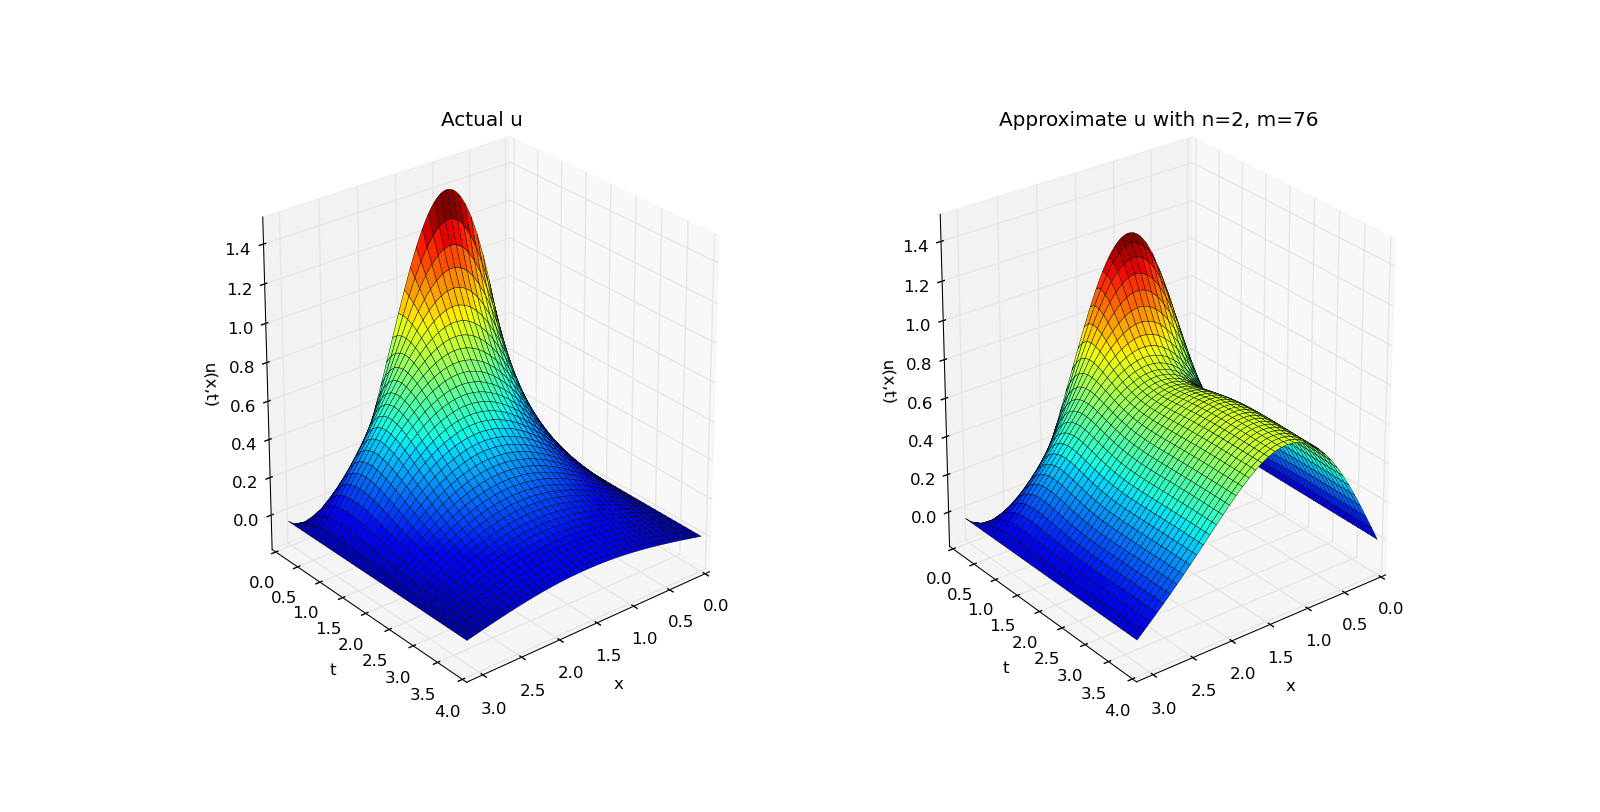
\includegraphics[trim = 6.5cm 1cm 6cm 2cm, width=\linewidth]{ProjectFiles/results/plots/n2m76.png} \\\vspace{2cm}
	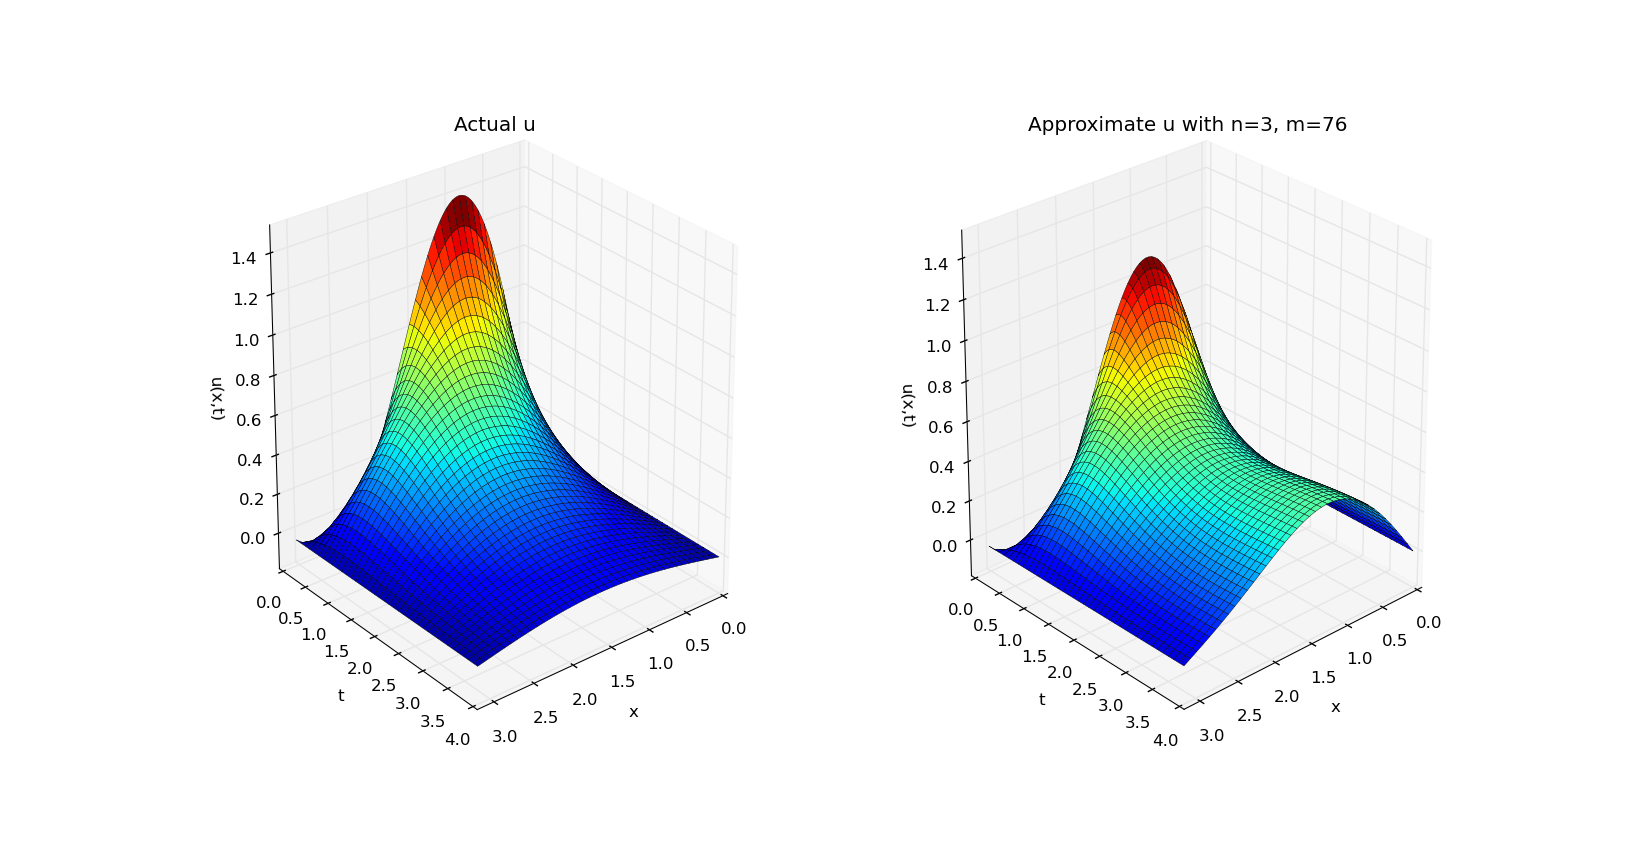
\includegraphics[trim = 6.5cm 3cm 6cm 2cm, width=\linewidth]{ProjectFiles/results/plots/n3m76.png} \\\vspace{2cm}
	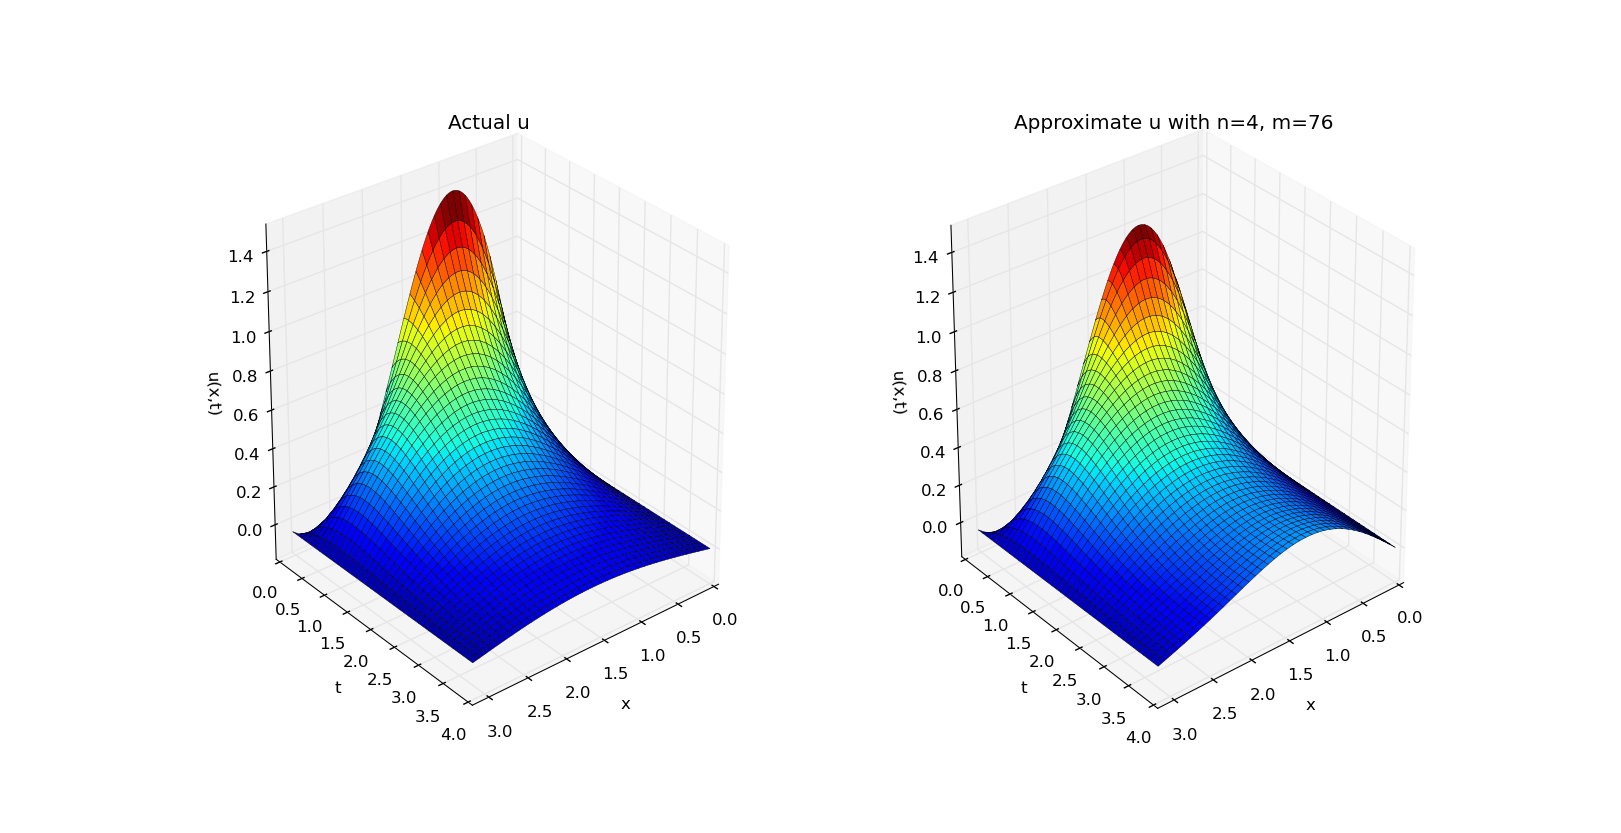
\includegraphics[trim = 6.5cm 3cm 6cm 2cm, width=\linewidth]{ProjectFiles/results/plots/n4m76.png} \\\vspace{2cm}
	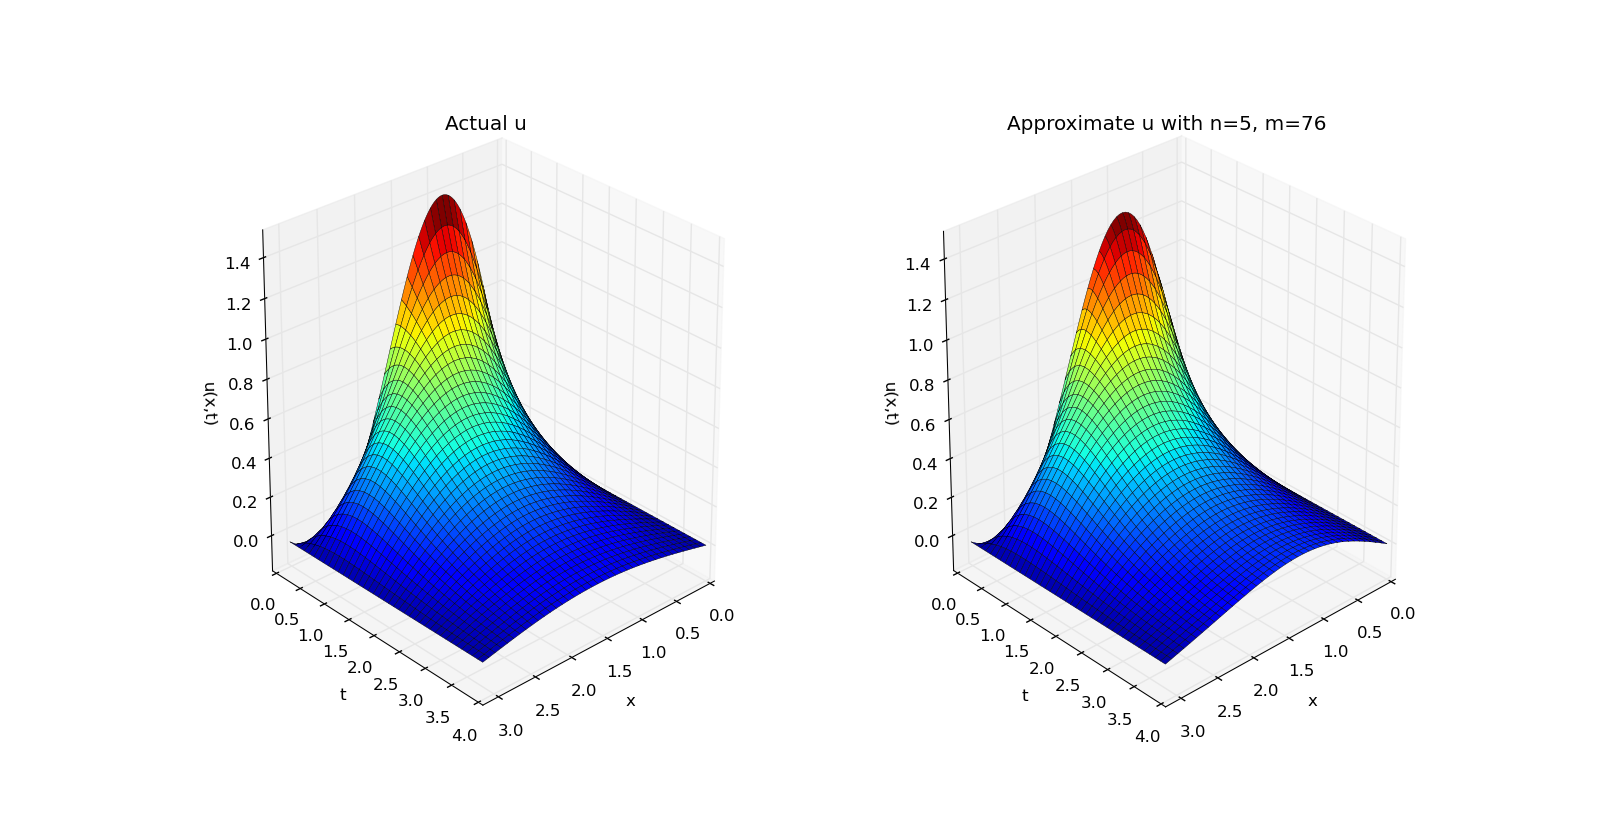
\includegraphics[trim = 6.5cm 3cm 6cm 2cm, width=\linewidth]{ProjectFiles/results/plots/n5m76.png} \\\vspace{2cm}
	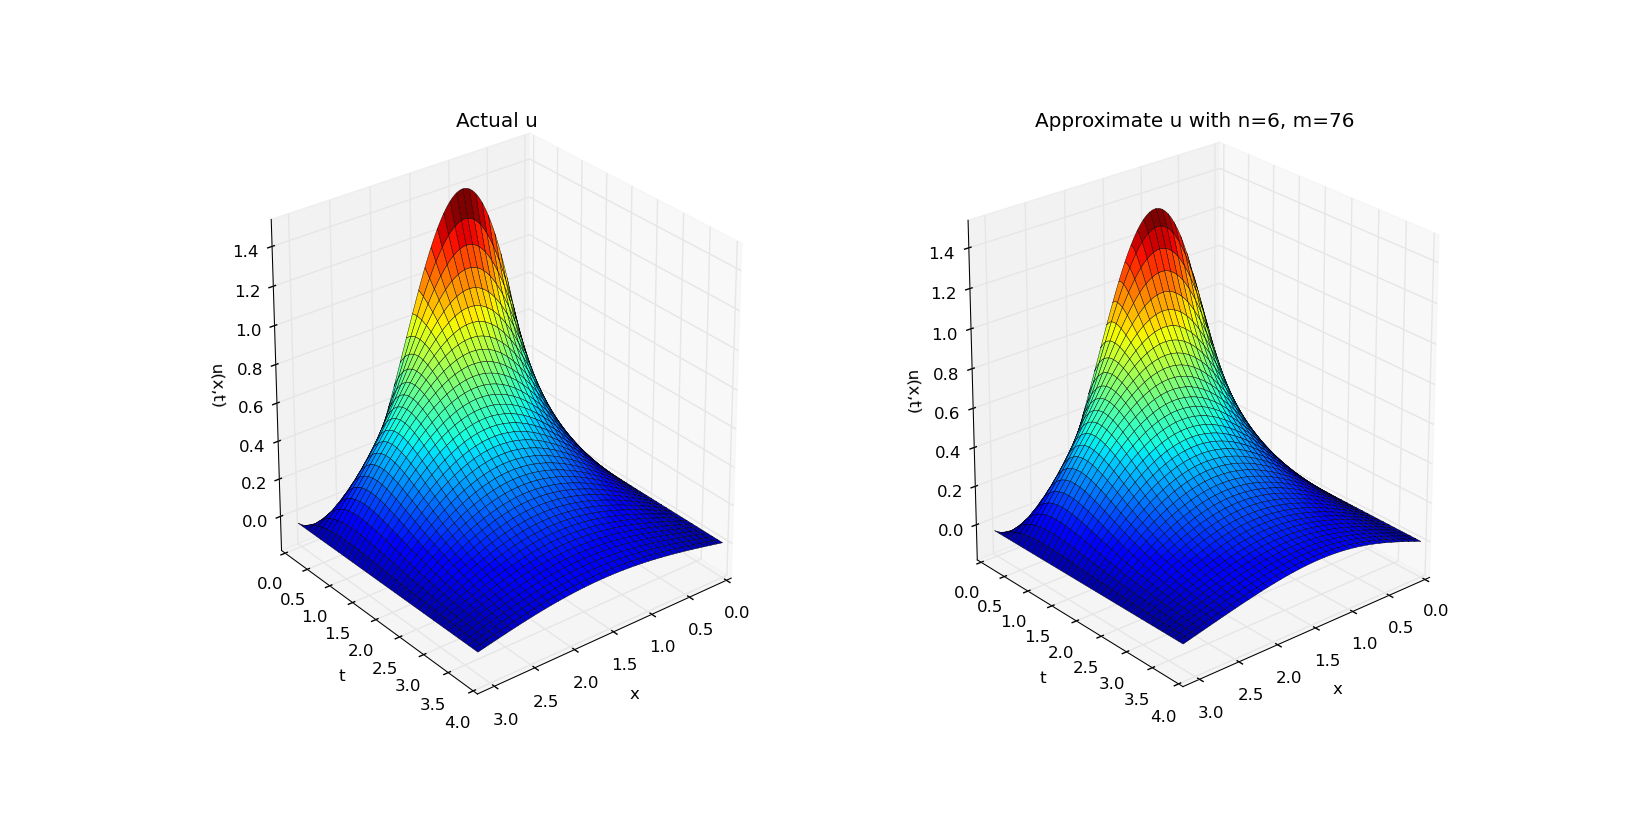
\includegraphics[trim = 6.5cm 3cm 6cm 2cm, width=\linewidth]{ProjectFiles/results/plots/n6m76.png} \\\vspace{2cm}
	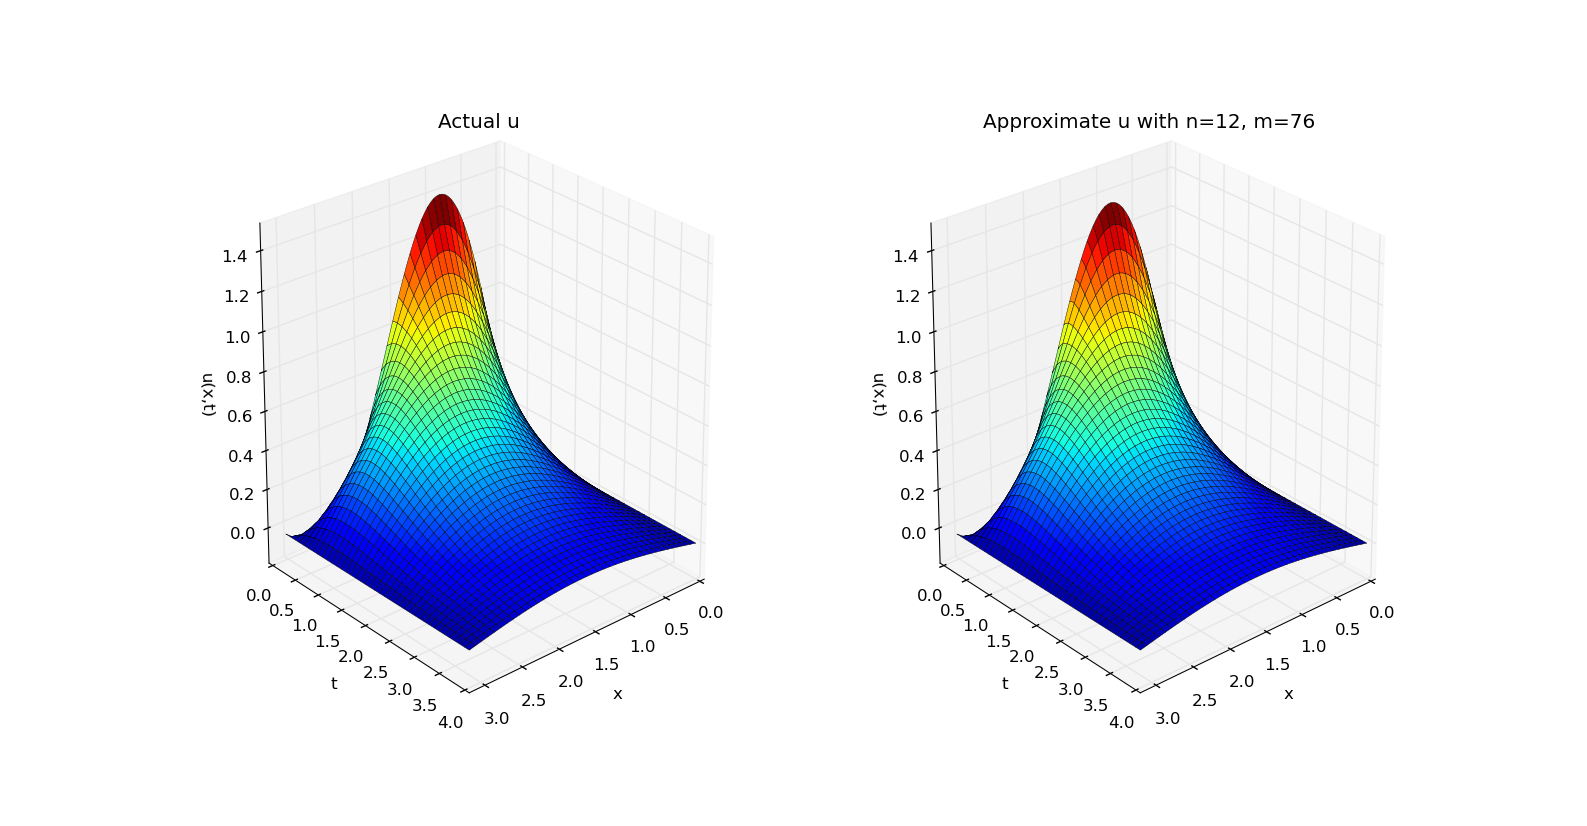
\includegraphics[trim = 6.5cm 3cm 6cm 2cm, width=\linewidth]{ProjectFiles/results/plots/n12m76.png} \\\vspace{2cm}
	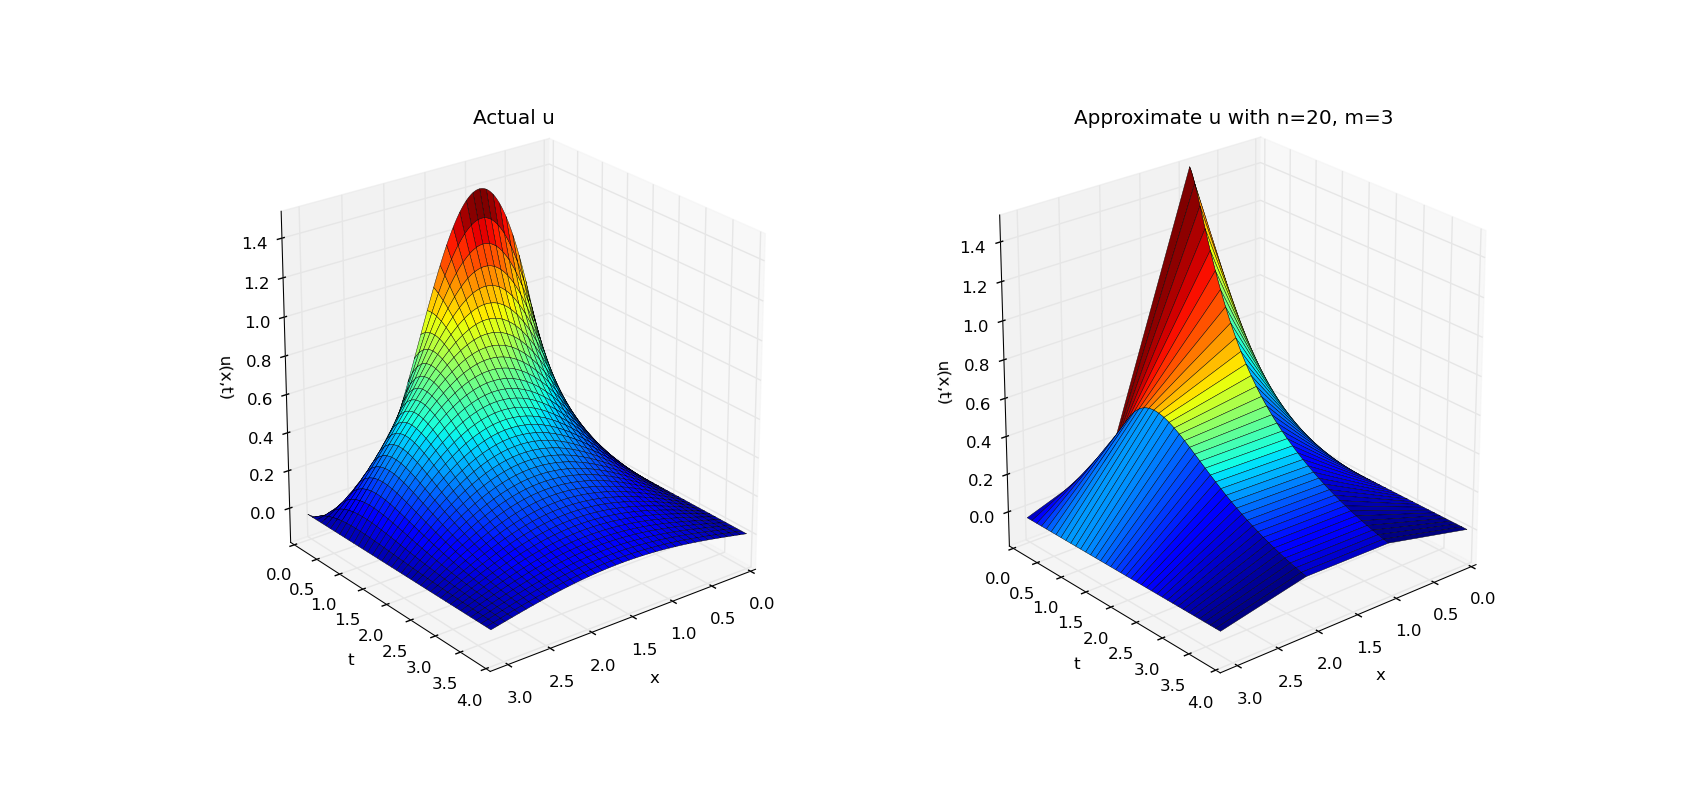
\includegraphics[trim = 6.5cm 3cm 6cm 2cm, width=\linewidth]{ProjectFiles/results/plots/n20m3.png} \\\vspace{2cm}
	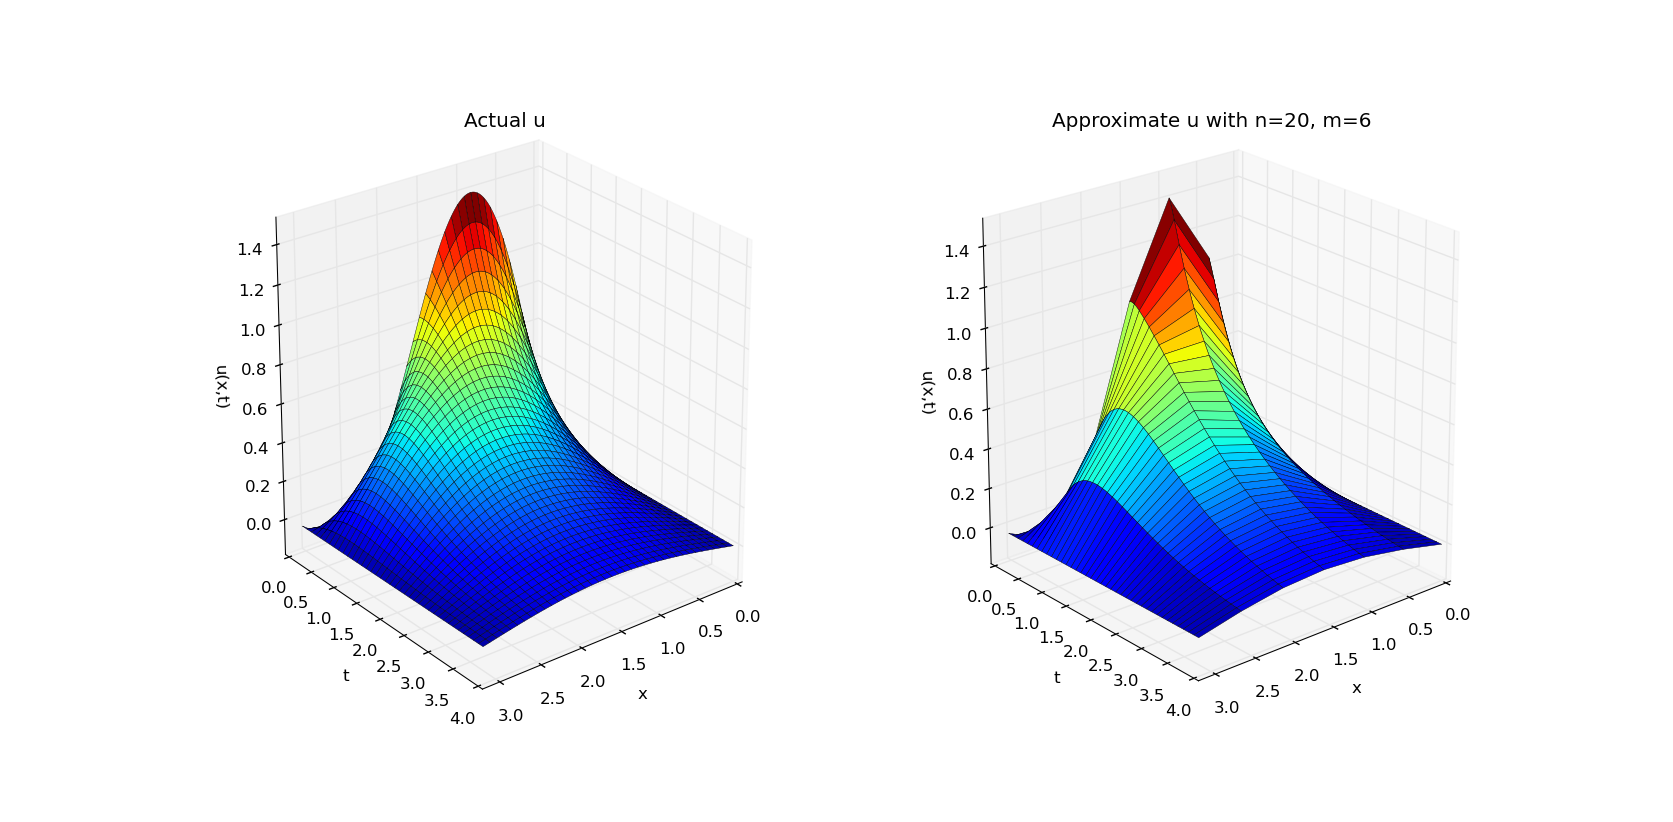
\includegraphics[trim = 6.5cm 3cm 6cm 2cm, width=\linewidth]{ProjectFiles/results/plots/n20m6.png} \\\vspace{2cm}
	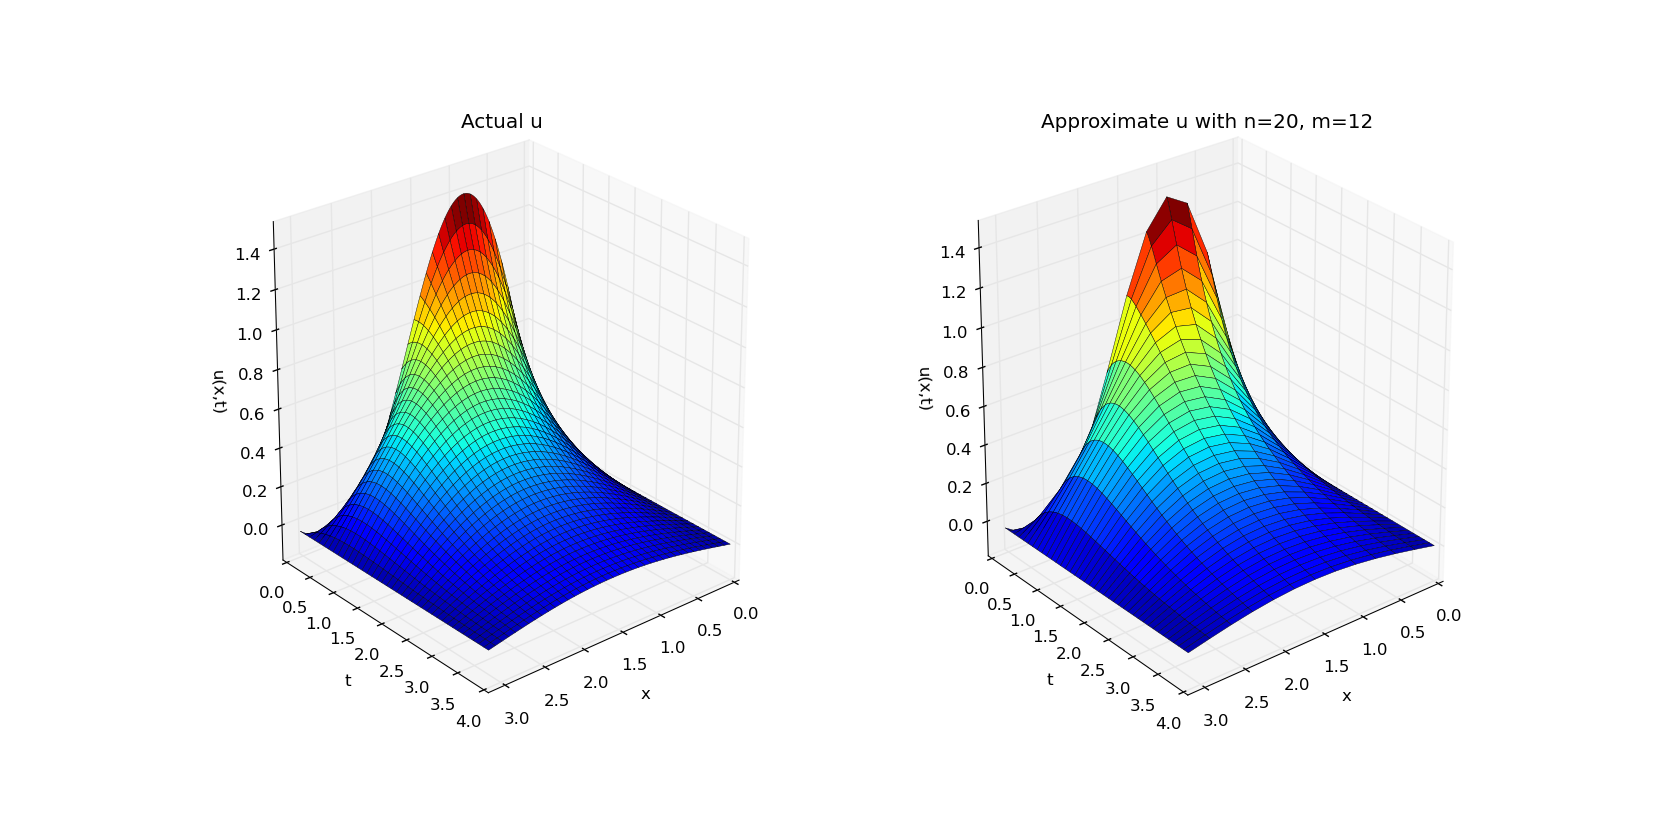
\includegraphics[trim = 6.5cm 3cm 6cm 2cm, width=\linewidth]{ProjectFiles/results/plots/n20m12.png} \\\vspace{2cm}
	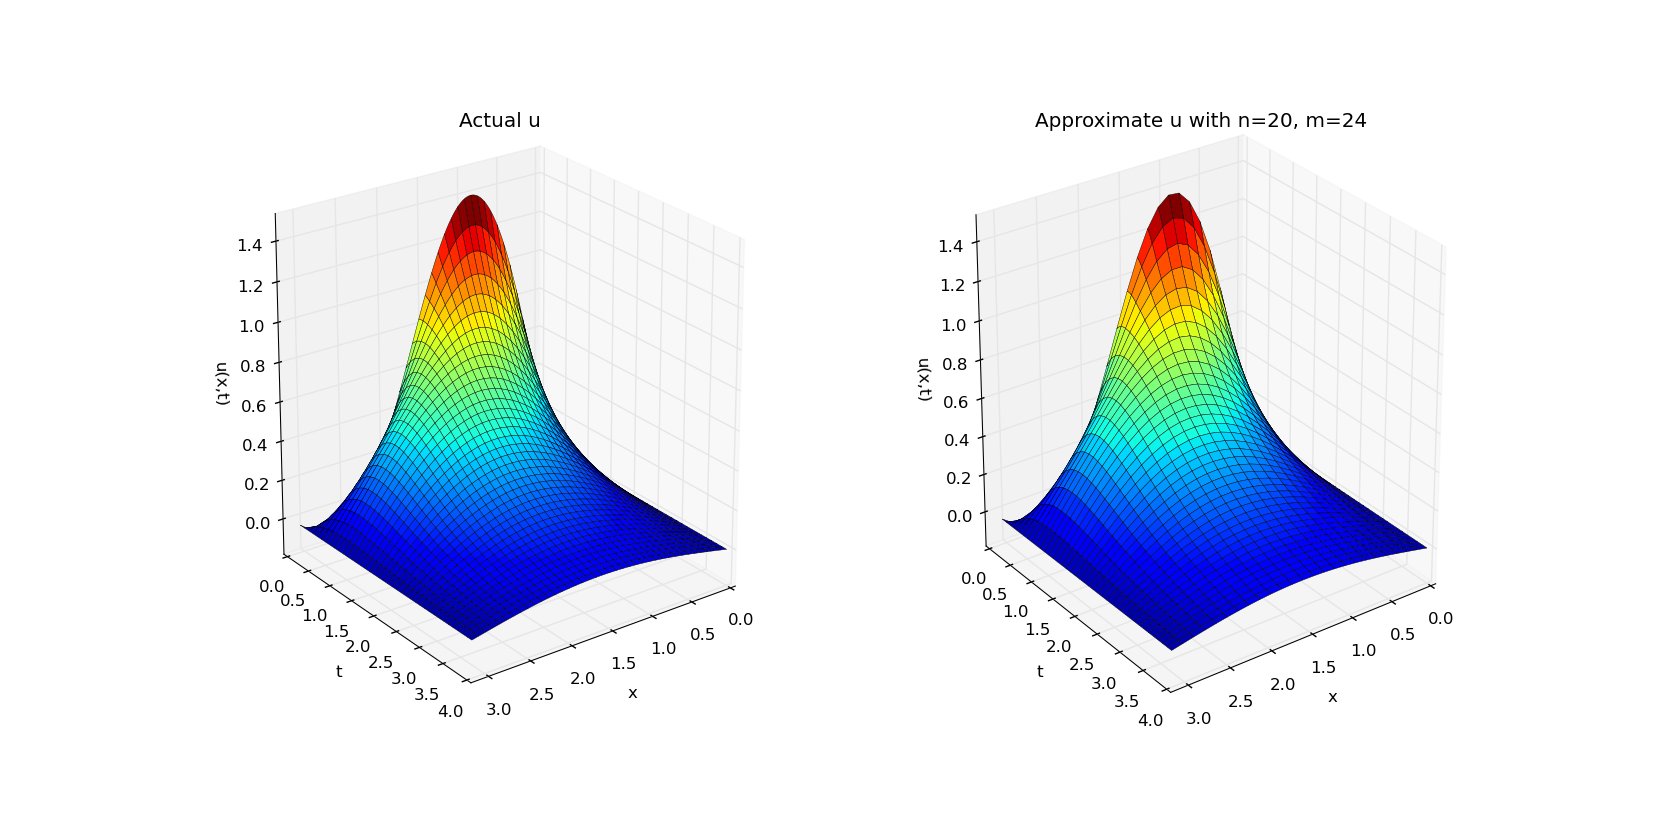
\includegraphics[trim = 6.5cm 3cm 6cm 2cm, width=\linewidth]{ProjectFiles/results/plots/n20m24.png} 
	
	\section*{Parallel Performance Analysis}
	The following tables and plots outline our parallel performance results for varying numbers of cores on both Mio and the Sayers Lab machines. Note that lg$(x)$ is our notation for $\log_2(x)$.
	
	\subsection*{Table 4} \small\textit{Number of cores vs. runtime(in seconds) for $N=50,000$\\ and $m=250,000$} \\\\
	\normalsize
	\begin{tabular}{r||r|r}
	\hline
		Cores              &Sayers Lab                     &Mio \\ 
	\hline
		  1.0      &3661.0877999999998      &2245.8103000000001 \\ 
		  2.0      &1918.2696000000001      &1182.6335999999999 \\ 
		  4.0               &1021.9571      &636.83158000000003 \\ 
		  8.0      &474.32260000000002               &348.26038 \\ 
		 16.0      &264.32758000000001      &164.24718999999999 \\ 
		 32.0               &153.50402      &80.234003999999999 \\ 
		 64.0      &84.893333999999996      &43.834428000000003 \\ 
		128.0                     &N/A      &21.293009999999999 \\ 
		256.0                     &N/A      &16.503080000000001 \\ 
		512.0                     &N/A      &23.166782000000001 \\ 
		\hline
	\end{tabular}
	
	\subsection*{Plot 1} \small\textit{Plot of Table $4$ data $(lg(cores)$ vs. $lg(runtime))$} \\
	\normalsize
	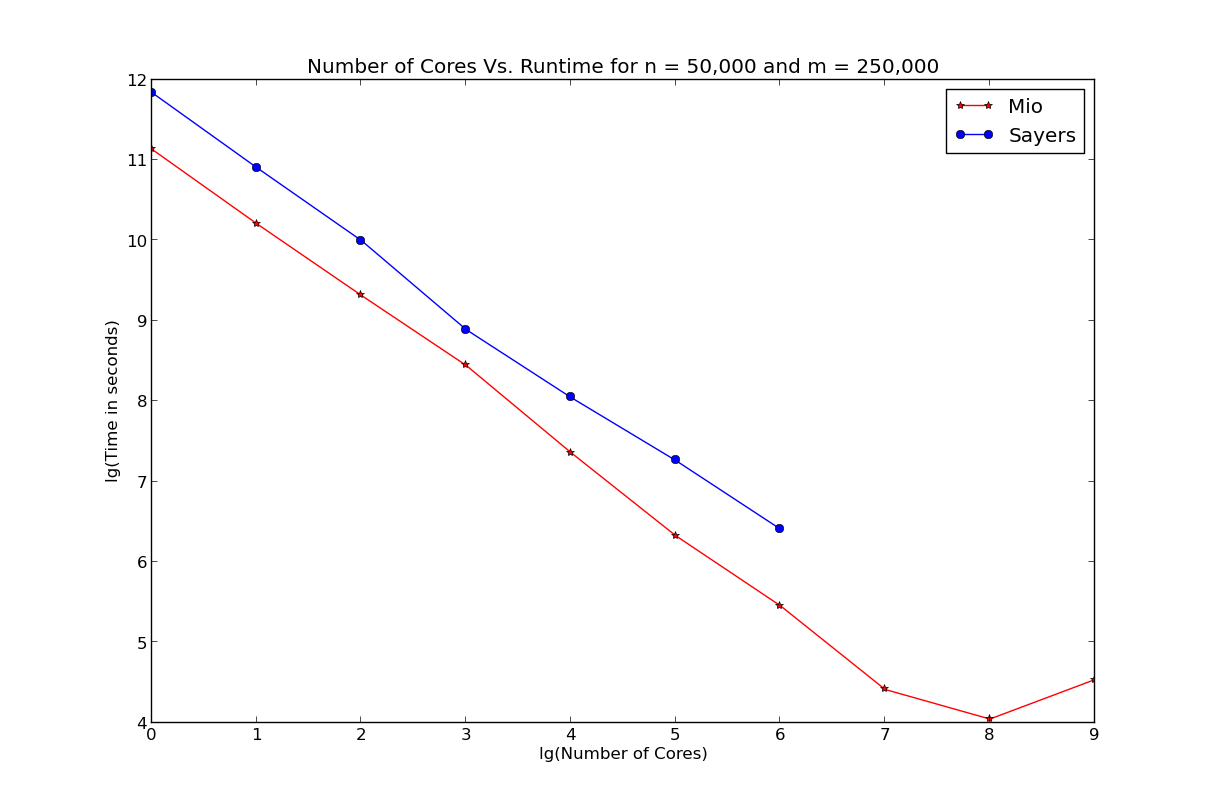
\includegraphics[width=.75\linewidth]{ProjectFiles/results/plots/coresVtime.png} \\
	Table 4 and Plot 1 show a clear linear correlation between number of processors and runtime on both Mio and Sayers Lab, up until 128 cores (on Mio). 256 cores still runs faster than 128 but the relative speedup is much less than that between lower numbers of cores. By 512 cores, the runtime actually begins to increase, suggesting a dominance of serial related processes, most likely communication beween processors. It is interesting to see that Mio is consistently faster than Sayers Lab for any number of course (of those tested). This is most likely due to the slightly better processors and much faster communication time between processors on Mio.
	
	\subsection*{Table 5} \small\textit{Number of cores vs. speedup for $N=50,000$ and $m=250,000$} \\\\
	\normalsize
	\begin{tabular}{r||r|r}
	\hline
  Cores              &Sayers Lab                     &Mio \\ 
	\hline
		  1.0                     &1.0                     &1.0 \\ 
		  2.0      &1.9085366311388137       &1.898990777870678 \\ 
		  4.0      &3.5824280686537624      &3.5265372675142777 \\ 
		  8.0       &7.718560743257858      &6.4486528728878092 \\ 
		 16.0      &13.850570568534692      &13.673355994705298 \\ 
		 32.0      &23.850110244669814      &27.990754393860239 \\ 
		 64.0      &43.125739413179367      &51.233936484810521 \\ 
		128.0                     &N/A      &105.47171583538449 \\ 
		256.0                     &N/A      &136.08431274646915 \\ 
		512.0                     &N/A      &96.940969185966352 \\ 
		\hline
	\end{tabular}
	
	\subsection*{Plot 2} \small\textit{Plot of Table $5$ data $(lg(cores)$ vs. $lg(speedup))$} \\
	\normalsize
	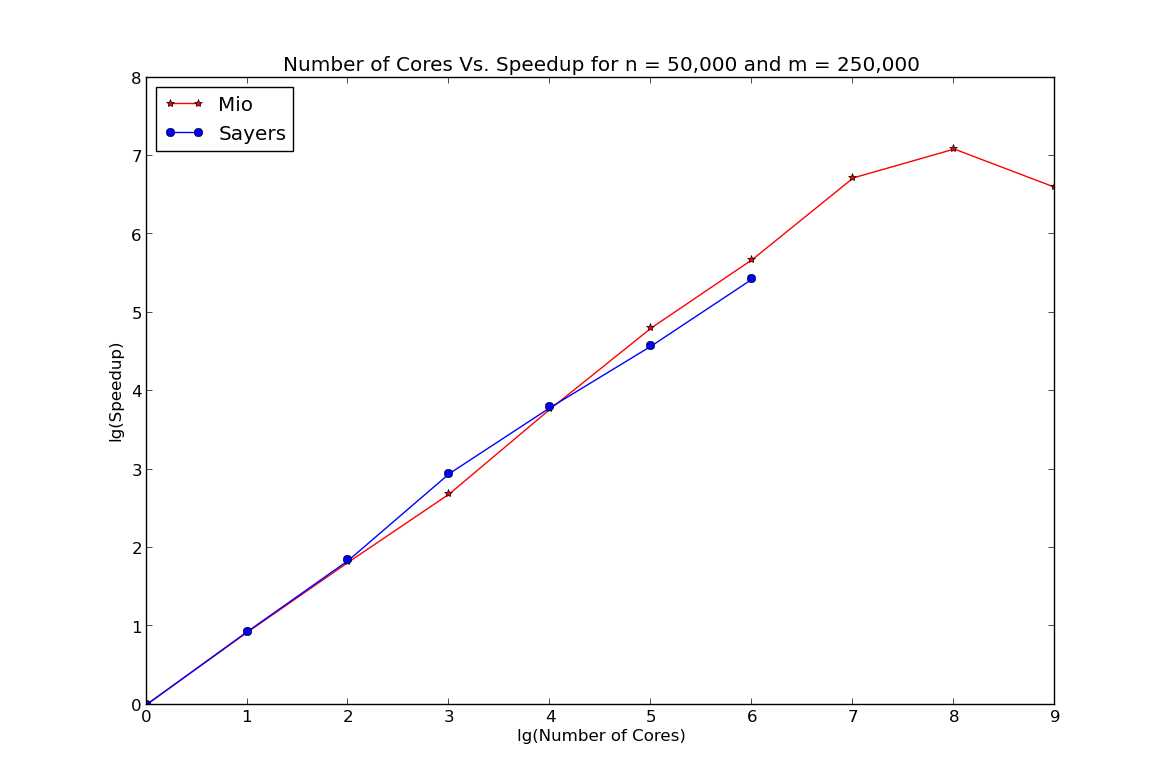
\includegraphics[width=.75\linewidth]{ProjectFiles/results/plots/coresVspeedup.png} \\
	Although Mio ran faster than Sayers Lab for every tested number of cores, the speedup data presented in Table 5 and Plot 2 is nearly identical for the two. For unknown reasons, Sayers Lab got incredible speedup for eight cores. As expected, Mio began to show better results in terms of speedup as the number of cores got large, most likely due to its superior InfiniBand connection. Even so, both machines showed linear speedup up to 64 cores on Sayers Lab and 128 cores on Mio.
	
	\subsection*{Table 6} \small\textit{Number of cores vs. efficiency for $N=50,000$ and $m=250,000$} \\\\
	\normalsize
	\begin{tabular}{r||r|r}
	\hline
		Cores              &Sayers Lab                     &Mio \\ 
	\hline
		  1.0                     &1.0                     &1.0 \\ 
		  2.0     &0.95426831556940683     &0.94949538893533902 \\ 
		  4.0      &0.8956070171634406     &0.88163431687856941 \\ 
		  8.0     &0.96482009290723225     &0.80608160911097615 \\ 
		 16.0     &0.86566066053341828     &0.85458474966908116 \\ 
		 32.0     &0.74531594514593169     &0.87471107480813248 \\ 
		 64.0     &0.67383967833092762     &0.80053025757516438 \\ 
		128.0                     &N/A      &0.8239977799639413 \\ 
		256.0                     &N/A     &0.53157934666589512 \\ 
		512.0                     &N/A     &0.18933783044134053 \\ 
		\hline
	\end{tabular}
	
	\subsection*{Plot 3} \small\textit{Plot of Table $6$ data $(lg(cores)$ vs. efficiency$)$} \\
	\normalsize
	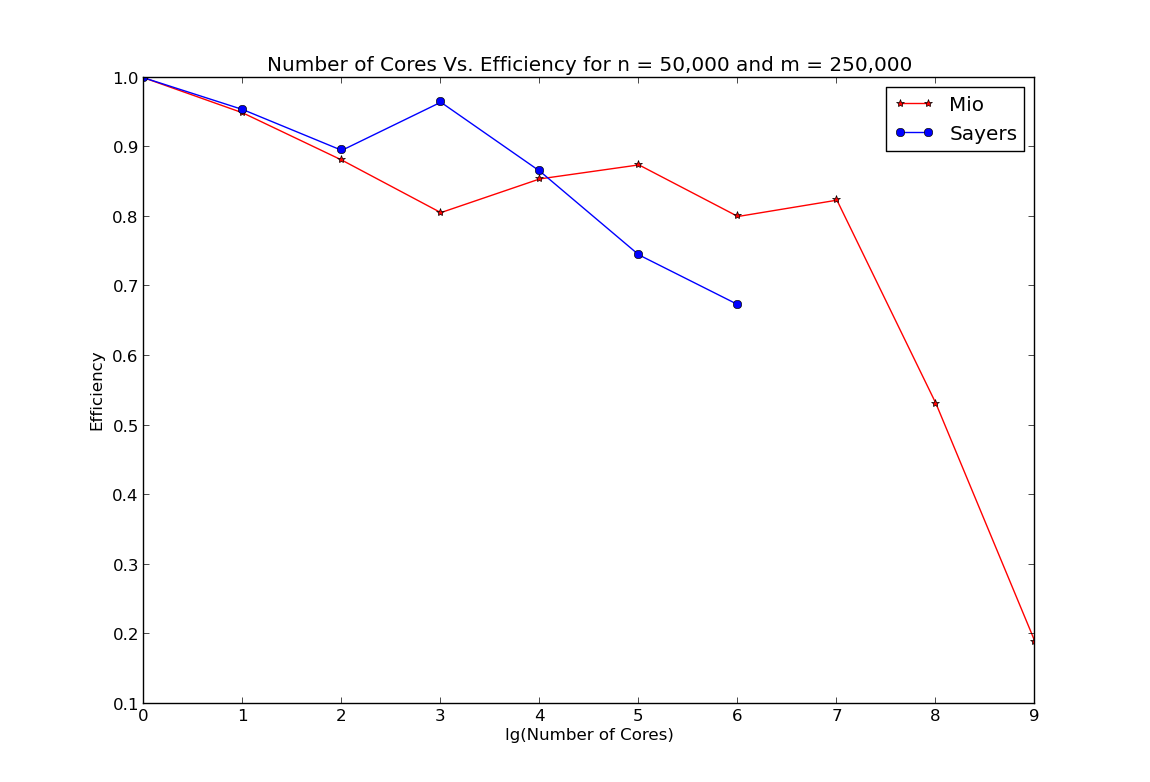
\includegraphics[width=.75\linewidth]{ProjectFiles/results/plots/coresVefficiency.png}
	
	\subsection*{Table 7} \small\textit{Number of cores vs. experimental serial fraction of the code for\\ $N=50,000$ and $m=250,000$} \\\\
	\normalsize
	\begin{tabular}{r||r|r}
	\hline
		Cores              &Sayers Lab                     &Mio \\ 
	\hline
		  2.0    &0.047923297551072164    &0.053191001929236759 \\ 
		  4.0     &0.03885371628253953    &0.044752372896321647 \\ 
		  8.0   &0.0052089514409975812    &0.034367025567564609 \\ 
		 16.0    &0.010345804508339492    &0.011343930518085162 \\ 
		 32.0     &0.01102299598743091   &0.0046204722317963586 \\ 
		 64.0   &0.0076830559693734967   &0.0039551114498611187 \\ 
		128.0                     &N/A   &0.0016818543519778373 \\ 
		256.0                     &N/A   &0.0034556341402023306 \\ 
		512.0                     &N/A   &0.0083787958735268026 \\ 
		\hline
	\end{tabular}
	
	\subsection*{Plot 4} \small\textit{Plot of Table $7$ data $(lg(cores)$ vs. experimental serial fraction of the code$)$} \\
	\normalsize
	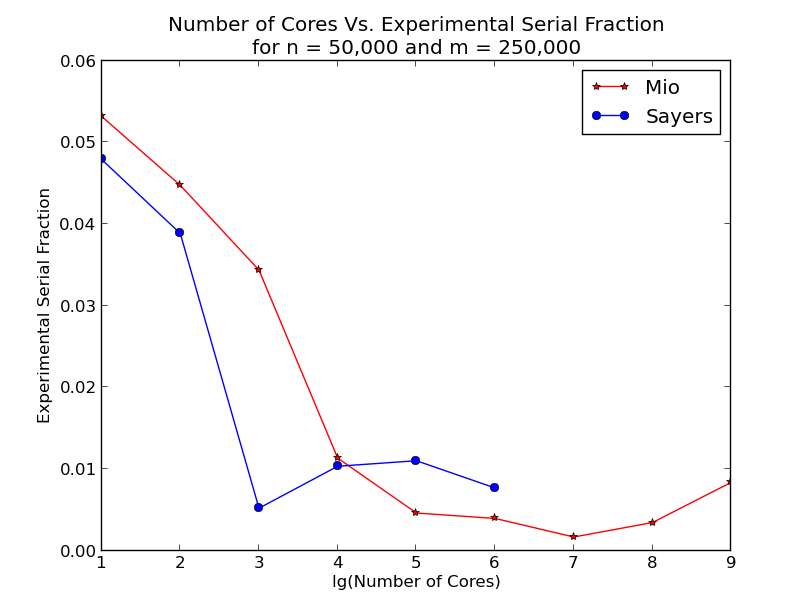
\includegraphics[width=.75\linewidth]{ProjectFiles/results/plots/coresVexpserialfrac.png}
	
	\begin{thebibliography}{1}
		\bibitem{sheen03}
			Dongwoo Sheen, Ian H. Sloan, and Vidar Thom\'{e}e,
			\emph{A parallel method for time discretization of parabolic equations based on Laplace transformation and quadrature}.
			IMA Journal of Numerical Analysis (2003) 23,
			269-299
			
	\end{thebibliography}
	
\end{document}
